% \IUref{IUAdmPS}{Administrar Planta de Selección}
% \IUref{IUModPS}{Modificar Planta de Selección}
% \IUref{IUEliPS}{Eliminar Planta de Selección}


% Copie este bloque por cada caso de uso:
%-------------------------------------- COMIENZA descripción del caso de uso.

%\begin{UseCase}[archivo de imágen]{UCX}{Nombre del Caso de uso}{
	\begin{UseCase}{CU23}{Moficar un curso}{
		Resumen:Cuando el Gerente de Sucursal va a Modificar un curso en el sistema, se ingresan los datos: numero de curso(id) o los datos generales como nombre de curso, costo, horario, fecha de inicio,area, fecha de termino,nombre de instructor y su  horario en formato 24:00.Una vez Validado los 8 campos,minimo el nombre de curso (obligatorio), se despliega una lista con las coincidencias,El gerente selccionara un curso con un boton para modificar datos en el sistema.	
		\begin{figure}
  		\centering
   		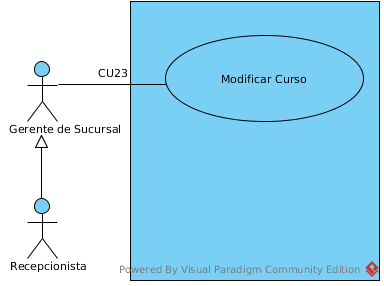
\includegraphics[width=0.4\textwidth]{images/CU23}
  		\caption{CU23 Modificar un curso}
		\end{figure}
	}
		\UCitem{Versión}{1.0}
		\UCitem{Actor}{Gerente de Sucursal}
		\UCitem{Propósito}{Modificacion de curso por el Gerente de Sucursal.}
		\UCitem{Entradas}{nombre de curso, costo, horario, fecha de inicio,area, fecha de termino,nombre de instructor y su  horario en formato 24:00}
		\UCitem{Origen}{Teclado}
		\UCitem{Salidas}{nombre de curso, costo, horario, fecha de inicio,area, fecha de termino,nombre de instructor y su  horario en formato 24:00 }
		\UCitem{Destino}{Pantalla}
		\UCitem{Precondiciones}{El curso debe de estar registrado en el sistema con las mismas descripciones.}
		\UCitem{Postcondiciones}{El Gerente de Sucursal modificara un curso a la base de datos del sistema.}
		\UCitem{Errores}{Que no se tenga ningun curso registrado.}
		\UCitem{Tipo}{Caso de uso primario}
		\UCitem{Observaciones}{Los cursos solo pueden ser Modificados por un Gerente de Sucursal.}
		\UCitem{Autor}{Carrillo Mendoza Martín Alejandro.}
		\UCitem{Reviso}{Carrillo Mendoza Martín Alejandro.}
	\end{UseCase}
	\newpage
	\begin{UCtrayectoria}{Principal}
	\UCpaso[\UCactor] Ingresa a la pagina web de \IUref{IU21.0}{Pantalla de Control de Acceso}\label{CU23.0Login} y proporciona su correspondiente nombre de usuario (username) y contraseña (password) para acceder al sistema.
		\UCpaso Válida que el actor se encuentre dado de alta en el sistema. Se utiliza la regla \BRref{BR117}{Determinar si el usuario tiene acceso al sistema.} \Trayref{A}.
	\UCpaso Despliega la pantalla {IU21.1}{Pantalla de acceso Gerente de Sucursal}
	\UCpaso[\UCactor] Al solicitar la modificacion de un curso a la base de datos,selecciona la pestaña " Modificar Curso  " de la IU21.1 de Menú principal.
	\UCpaso El sistema carga una nueva pagina{IU23.1}{Pantalla de Modificar Curso} con los campos: nombre de curso, costo, horario, fecha de inicio,area, fecha de termino,nombre de instructor y su  horario en formato 24:00.
	\UCpaso[\UCactor] Introduce los datos del curso a modificar, con su respetivo formato y tipo de dato solicitado, estos son: nombre de curso(varchar), costo(float), fecha de inicio(DATE), fecha de termino(DATE), costo(float)todos ellos obligatorios para la modificaion de un curso en el sistema.
    \UCpaso[\UCactor] Selecciona el nombre del instructor a impartir nuevo curso.
	\UCpaso[\UCactor] Selecciona los dias ala semana en los que se imparte nuevo curso.
	\UCpaso[\UCactor] Selecciona la hora en que se impartira un curso (los dias ya seleccionados previamente).
	\UCpaso[\UCactor] Selecciona el area donde se impartira un curso.
	\UCpaso[\UCactor] Confirma la modificacion de curso al sistema dando click al boton \IUbutton{Enviar} de \label{IU23.1 Modificar Curso}.
	\UCpaso Verifica que todos los campos esten llenos ademas con el formato y tipo correspondiente a los datos ubucados en la base de datos. \BRref{BR118}{Validar los datos de un formulario} \Trayref{B}
		\UCpaso Consulta los datos proporcionados a la base e imprime los cursos con la descripcion exacta de el numero de curso, o en su defecto los datos generales del curso a Modificar.
	\UCpaso[\UCactor] Confirma con el boton "Modificar." curso al al sistema.
	\UCpaso El sistema nos abre una nueva pagina donde se despliegan todos los campos del curso a modificar.
	UCpaso[\UCactor] Modifica los datos del curso colocando el raton en el campo a modificar. campos seleccionables son :numero de curso, nombre de curso, costo, horario, fecha de inicio,area, fecha de termino,nombre de instructor y su  horario en formato 24:00.
	\UCpaso[\UCactor] Confirma la Modificacion de Curso con el boton Guardar cambios.
		\UCpaso Muestra el \IUref{UI23}{Modificacion Exitosa de curso.}\Trayref{C}.
		\UCpaso Regresa a la pantalla principal de acceso a gerente de sucursal\IUref{IU21.1}{Pantalla de acceso a Gerente de Sucursal}.
\end{UCtrayectoria}

\begin{UCtrayectoriaA}{A}{El actor no introduce nombre de usuario (username) y contraseña (password) para poder ingresar al sistema.}
			\UCpaso Muestra el mensaje {\bf MSG23.0-}``Usuario [{\em y/o}] contraseñas no validos.''.
			\UCpaso[\UCactor] Oprimé el botón \IUbutton{Aceptar}.
			\UCpaso Regresa a la pantalla principal de acceso a gerente de sucursal\IUref{IU21.1}{Pantalla de acceso a Gerente de Sucursal}.
		\end{UCtrayectoriaA}

		\begin{UCtrayectoriaA}{B}{Almenos un campo no esta lleno o no tiene formato adecuado}
			\UCpaso Muestra el mensaje {\bf MSG23.1-}``Uno o más [{\em campos}] no tienen el formato adecuado''.ademas que se tiene obligatoriamente que llenar todos los campos.
			\UCpaso[\UCactor] Oprime el botón \IUbutton{Aceptar}
			\UCpaso[] Termina el caso de uso.
		\end{UCtrayectoriaA}
		
		\begin{UCtrayectoriaA}{C}{La modificacion del curso no fue realizada }
			\UCpaso Muestra el Mensaje {\bf MSG23.2-}El Curso [{\em nombre de curso, costo, horario, fecha de inicio,area, fecha de termino,nombre de instructor y su  horario en formato 24:00 }] no registrado en el sistema, compruebe memoria en el Disco.
			\UCpaso[\UCactor] Oprime el botón \IUbutton{Aceptar}
			\UCpaso[] Termina el caso de uso.
		\end{UCtrayectoriaA}	
%-------------------------------------- TERMINA descripción del caso de uso.